\documentclass[aspectratio=169]{beamer}

% Theme and Color Setup
\usetheme{Madrid}
\usecolortheme{whale}
\useinnertheme{rectangles}
\useoutertheme{miniframes}

% Additional Packages
\usepackage[utf8]{inputenc}
\usepackage[T1]{fontenc}
\usepackage{graphicx}
\usepackage{booktabs}
\usepackage{listings}
\usepackage{amsmath}
\usepackage{amssymb}
\usepackage{xcolor}
\usepackage{tikz}
\usepackage{pgfplots}
\pgfplotsset{compat=1.18}
\usetikzlibrary{positioning}
\usepackage{hyperref}

% Custom Colors
\definecolor{myblue}{RGB}{31, 73, 125}
\definecolor{mygray}{RGB}{100, 100, 100}
\definecolor{mygreen}{RGB}{0, 128, 0}
\definecolor{myorange}{RGB}{230, 126, 34}
\definecolor{mycodebackground}{RGB}{245, 245, 245}

% Set Theme Colors
\setbeamercolor{structure}{fg=myblue}
\setbeamercolor{frametitle}{fg=white, bg=myblue}
\setbeamercolor{title}{fg=myblue}
\setbeamercolor{section in toc}{fg=myblue}
\setbeamercolor{item projected}{fg=white, bg=myblue}
\setbeamercolor{block title}{bg=myblue!20, fg=myblue}
\setbeamercolor{block body}{bg=myblue!10}
\setbeamercolor{alerted text}{fg=myorange}

% Set Fonts
\setbeamerfont{title}{size=\Large, series=\bfseries}
\setbeamerfont{frametitle}{size=\large, series=\bfseries}
\setbeamerfont{caption}{size=\small}
\setbeamerfont{footnote}{size=\tiny}

% Code Listing Style
\lstdefinestyle{customcode}{
  backgroundcolor=\color{mycodebackground},
  basicstyle=\footnotesize\ttfamily,
  breakatwhitespace=false,
  breaklines=true,
  commentstyle=\color{mygreen}\itshape,
  keywordstyle=\color{blue}\bfseries,
  stringstyle=\color{myorange},
  numbers=left,
  numbersep=8pt,
  numberstyle=\tiny\color{mygray},
  frame=single,
  framesep=5pt,
  rulecolor=\color{mygray},
  showspaces=false,
  showstringspaces=false,
  showtabs=false,
  tabsize=2,
  captionpos=b
}
\lstset{style=customcode}

% Custom Commands
\newcommand{\hilight}[1]{\colorbox{myorange!30}{#1}}
\newcommand{\source}[1]{\vspace{0.2cm}\hfill{\tiny\textcolor{mygray}{Source: #1}}}
\newcommand{\concept}[1]{\textcolor{myblue}{\textbf{#1}}}
\newcommand{\separator}{\begin{center}\rule{0.5\linewidth}{0.5pt}\end{center}}

% Footer and Navigation Setup
\setbeamertemplate{footline}{
  \leavevmode%
  \hbox{%
  \begin{beamercolorbox}[wd=.3\paperwidth,ht=2.25ex,dp=1ex,center]{author in head/foot}%
    \usebeamerfont{author in head/foot}\insertshortauthor
  \end{beamercolorbox}%
  \begin{beamercolorbox}[wd=.5\paperwidth,ht=2.25ex,dp=1ex,center]{title in head/foot}%
    \usebeamerfont{title in head/foot}\insertshorttitle
  \end{beamercolorbox}%
  \begin{beamercolorbox}[wd=.2\paperwidth,ht=2.25ex,dp=1ex,center]{date in head/foot}%
    \usebeamerfont{date in head/foot}
    \insertframenumber{} / \inserttotalframenumber
  \end{beamercolorbox}}%
  \vskip0pt%
}

% Turn off navigation symbols
\setbeamertemplate{navigation symbols}{}

% Document Start
\begin{document}

% Title Frame
\begin{frame}[fragile]
  \titlepage
\end{frame}

% Table of Contents
\begin{frame}[fragile]{Presentation Overview}
  \tableofcontents[hideallsubsections]
\end{frame}

% Section 1
\section{Basic Slide Layouts}

\begin{frame}[fragile]{Standard Text Frame}
  \begin{block}{Block Title Example}
    This shows a standard block element for important content or definitions.
  \end{block}
  
  \begin{itemize}
    \item Standard bullet points for main ideas
    \item Use \concept{concept highlighting} for important terms
    \item Secondary level points:
    \begin{itemize}
      \item Supporting details or explanations
      \item Additional examples or evidence
    \end{itemize}
    \item Use \hilight{highlight command} to emphasize key phrases
  \end{itemize}
  
  \begin{alertblock}{Important Note}
    Alert blocks can be used for critical information or warnings.
  \end{alertblock}
\end{frame}

\begin{frame}[fragile]{Two-Column Layout}
  \begin{columns}
    \begin{column}{0.48\textwidth}
      \begin{block}{Left Column}
        Use columns for comparing ideas or presenting related content side by side.
        \begin{itemize}
          \item Point 1
          \item Point 2
          \item Point 3
        \end{itemize}
      \end{block}
    \end{column}
    
    \begin{column}{0.48\textwidth}
      \begin{block}{Right Column}
        The width of columns can be adjusted based on content needs.
        \begin{itemize}
          \item Item A
          \item Item B
          \item Item C
        \end{itemize}
      \end{block}
    \end{column}
  \end{columns}
  
  \separator
  
  Text below columns spans the full width of the slide.
\end{frame}

% Section 2
\section{Visual Elements}

\begin{frame}[fragile]{Tables and Figures}
  \begin{columns}
    \begin{column}{0.48\textwidth}
      \begin{table}
        \centering
        \begin{tabular}{lcc}
          \toprule
          \textbf{Category} & \textbf{Value 1} & \textbf{Value 2} \\
          \midrule
          Item A & 42.5 & 18.3 \\
          Item B & 37.8 & 24.6 \\
          Item C & 25.3 & 31.2 \\
          \bottomrule
        \end{tabular}
        \caption{Example table with booktabs style}
      \end{table}
    \end{column}
    
    \begin{column}{0.48\textwidth}
      \centering
      % Replace with actual image file when available
      \fbox{\parbox{0.8\textwidth}{\centering Sample Image\\Placeholder}}
      \captionof{figure}{Sample figure with caption}
      \source{Citation or source information}
    \end{column}
  \end{columns}
\end{frame}

\begin{frame}[fragile]{Charts and Diagrams}
  \centering
  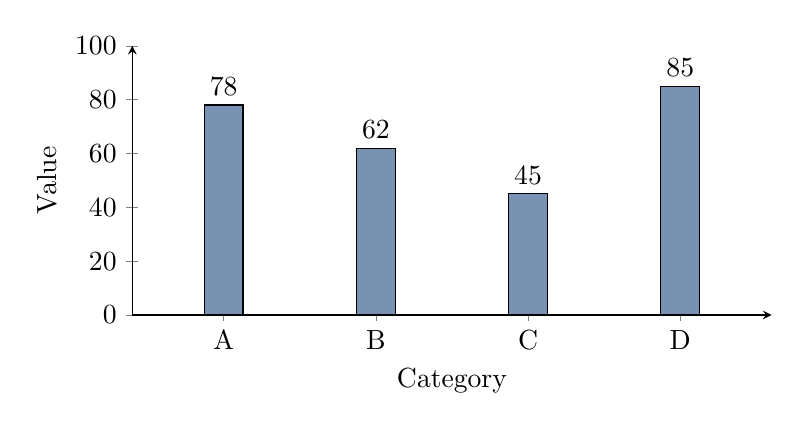
\begin{tikzpicture}
    \begin{axis}[
        width=0.8\textwidth,
        height=5cm,
        ybar,
        bar width=14pt,
        ylabel={Value},
        xlabel={Category},
        symbolic x coords={A, B, C, D},
        xtick=data,
        nodes near coords,
        ymin=0,
        ymax=100,
        axis lines=left,
        enlarge x limits=0.2,
        ylabel near ticks
      ]
      \addplot[fill=myblue!60] coordinates {
        (A, 78)
        (B, 62)
        (C, 45)
        (D, 85)
      };
    \end{axis}
  \end{tikzpicture}
  
  \vspace{0.5cm}
  
  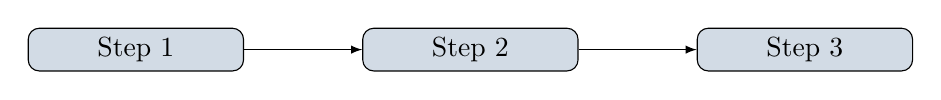
\begin{tikzpicture}[node distance=1.5cm]
    \node[draw, rounded corners, fill=myblue!20, text width=2.5cm, align=center] (a) {Step 1};
    \node[draw, rounded corners, fill=myblue!20, text width=2.5cm, align=center, right=of a] (b) {Step 2};
    \node[draw, rounded corners, fill=myblue!20, text width=2.5cm, align=center, right=of b] (c) {Step 3};
    
    \draw[-latex] (a) -- (b);
    \draw[-latex] (b) -- (c);
  \end{tikzpicture}
\end{frame}

% Section 3
\section{Technical Content}

\begin{frame}[fragile]{Code Examples}
  \begin{columns}
    \begin{column}{0.48\textwidth}
      \begin{lstlisting}[language=Python, caption=Sample Python code]
# Function example
def calculate_stats(data):
    """Calculate basic statistics"""
    results = {
        'mean': sum(data) / len(data),
        'max': max(data),
        'min': min(data)
    }
    return results
    
# Example call
data = [12, 45, 33, 27, 19]
stats = calculate_stats(data)
print(f"Mean: {stats['mean']}")
      \end{lstlisting}
    \end{column}
    
    \begin{column}{0.48\textwidth}
      Code can be displayed with:
      \begin{itemize}
        \item Syntax highlighting
        \item Line numbers
        \item Custom background
        \item Caption and title
      \end{itemize}
      
      \begin{block}{Key Points}
        Keep code examples concise and focused on the important concepts.
      \end{block}
    \end{column}
  \end{columns}
\end{frame}

\begin{frame}[fragile]{Mathematical Notation}
  \begin{block}{Equation Example}
    The relationship between variables can be expressed as:
    
    \begin{equation}
      f(x) = \alpha \cdot x^2 + \beta \cdot x + \gamma
    \end{equation}
    
    Where:
    \begin{itemize}
      \item $\alpha, \beta, \gamma$ are constants
      \item $x$ is the independent variable
    \end{itemize}
  \end{block}
  
  \begin{columns}
    \begin{column}{0.48\textwidth}
      Inline math examples:
      \begin{itemize}
        \item The integral $\int_{a}^{b} f(x) dx$ represents area
        \item For any $n > 0$, we have $\sum_{i=1}^{n} i = \frac{n(n+1)}{2}$
      \end{itemize}
    \end{column}
    
    \begin{column}{0.48\textwidth}
      Matrix notation:
      \begin{equation}
        A = \begin{bmatrix}
          a_{11} & a_{12} & a_{13} \\
          a_{21} & a_{22} & a_{23} \\
          a_{31} & a_{32} & a_{33}
        \end{bmatrix}
      \end{equation}
    \end{column}
  \end{columns}
\end{frame}

% Section 4
\section{Reference Slides}

\begin{frame}[fragile]{References and Citations}
  \begin{block}{Selected References}
    \footnotesize
    \begin{thebibliography}{9}
      \bibitem{ref1} Smith, J., and Johnson, A. (2023). Title of the paper. \textit{Journal Name}, 12(3), 45-67.
      
      \bibitem{ref2} Williams, S. (2022). Book title. Publisher Name.
      
      \bibitem{ref3} Brown, R., and Davis, M. (2021). Chapter title. In Editor Name (Ed.), \textit{Book Title} (pp. 123-145). Publisher.
    \end{thebibliography}
  \end{block}
  
  In-text citation examples:
  \begin{itemize}
    \item According to Smith and Johnson \cite{ref1}, the results indicate...
    \item This approach has been validated in previous studies \cite{ref2, ref3}.
  \end{itemize}
\end{frame}

\begin{frame}[fragile,plain]{Thank You Slide}
  \begin{center}
    \vspace{1cm}
    {\Large Thank You}
    
    \vspace{0.5cm}
    {\large Questions and Discussion}
    
    \vspace{1.5cm}
    {\small
    Email: email@university.edu\\
    \vspace{0.2cm}
    Twitter: @academichandle\\
    Website: www.university.edu}
  \end{center}
\end{frame}

\appendix

\begin{frame}[fragile]{Template Usage Notes}
  \begin{block}{How to Use This Template}
    \begin{itemize}
      \item Replace placeholder text with your content
      \item Update title page information
      \item Replace example images with your figures
      \item Adjust colors in the preamble if needed
    \end{itemize}
  \end{block}
  
  \begin{alertblock}{Important Tips}
    \begin{itemize}
      \item Keep slides concise (aim for 1 main idea per slide)
      \item Use consistent visual style throughout
      \item Test your presentation on the display you will use
      \item Consider creating a handout version
    \end{itemize}
  \end{block}
  
  \begin{block}{Custom Commands}
    \begin{itemize}
      \item \texttt{\textbackslash concept\{text\}} - Blue highlighted concept
      \item \texttt{\textbackslash hilight\{text\}} - Orange background highlight
      \item \texttt{\textbackslash source\{citation\}} - Small source citation
      \item \texttt{\textbackslash separator} - Horizontal rule
    \end{itemize}
  \end{block}
\end{frame}

\end{document}